\documentclass[tikz,border=50mm]{standalone}
% !TeX program = luatex

%===This is the preambule I call in every file===

\usepackage{tikz}
\usepackage{xcolor}
\usepackage{pgfplots}
\usepackage{circuitikz}
\usepackage{tikz-3dplot}
\pgfplotsset{compat=newest}
\usetikzlibrary{arrows.meta, shapes.geometric, positioning, perspective, patterns.meta, decorations.pathreplacing, decorations.pathmorphing, decorations.markings, patterns, arrows.meta, shapes, shapes.geometric, decorations.text, angles, quotes,calc, 3d, math, circuits.ee.IEC,hobby, knots, intersections, through}


%=== The Euler Med Logo ===
%=== i.e. My signature ===

\usepackage{amsmath, amsfonts}
\makeatletter
\newcommand*\eulermed{{
\scalebox{3.3}{$\mathbb{E}$}\kern-1pt \scalebox{1.5}{u$\ell\varepsilon\rho$}\kern-55pt
\raisebox{19pt}{\scalebox{1.5}{$\mathcal{M}\varepsilon\delta$}}}
\@}
\makeatother

\begin{document}
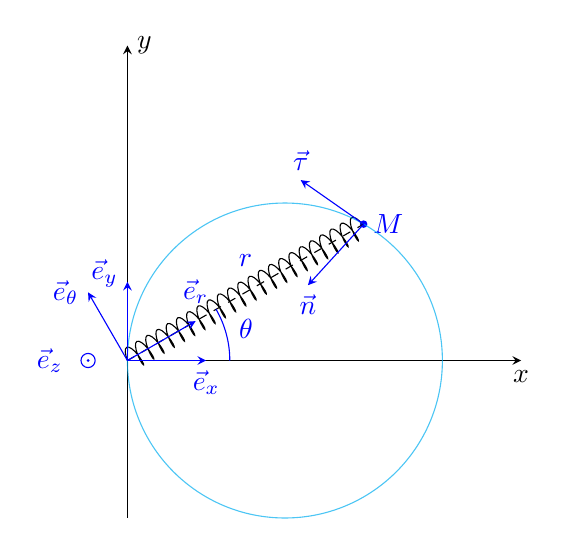
\begin{tikzpicture}[>=stealth]
%So I first want to locate my studied materiel point M, so I shifted the origin to (2,0) and mark M(m) using it's polar coordinates (r=2, theta=60) in TikZ (60:2).
\begin{scope}[shift={(2,0)}]
\coordinate(m) at (60:2);
\filldraw[blue] (m)circle(0.04) node[right]{$M$};
\end{scope}
%Now I have m it's going to be easy to draw everything related to it, here I've drawn the spring attached to it 
\draw[decoration={aspect=0.25, segment length=1.5mm, amplitude=1.5mm,coil},decorate] (0,0) -- (m);
%the axis
\draw[->] (0,0)--(5,0) node[below] {$x$};
\draw[->] (0,-2)--(0,4) node[right] {$y$};
%the trajectory of M which is a circle of radius 2 
\draw[cyan, opacity=0.7] (2,0) circle(2);
\begin{scope}[shift={(2,0)}]
%Frenet base 
\draw[dashed] (-2,0)--(60:2) node[midway, above=0.2, blue]{$r$};
\draw[->, blue] (m)--(73:1) node[below] {$\vec{n}$};
\draw[->, blue] (m)--(85:2.3) node[above] {$\vec{\tau}$};
\end{scope}
%marking the coordinates to draw the angle theta
\coordinate(o) at (0,0);
\coordinate(x) at (5,0);
\pic[ draw,inner sep=1pt, circle, blue, draw,angle 
eccentricity=1.2,"$\theta$", angle radius = 13mm] {angle = x--o--m};
%the polar and cartesian base
\draw[->, blue] (0,0)--(30:1) node[above=0.1] {$\vec{e}_r$};
\draw[->, blue] (0,0)--(120:1) node[left] {$\vec{e}_\theta$};
\draw[->, blue] (0,0)--(0,1) node[above=0.1, left] {$\vec{e}_y$};
\draw[->, blue] (0,0)--(1,0) node[below] {$\vec{e}_x$};
\draw[->, blue] (-0.5,0) circle(0.09);
\filldraw[blue] (-0.5,0)circle(0.009);
\node[blue, left] at (-0.7,0) {$\vec{e}_z$};
\end{tikzpicture}
\end{document}
